\documentclass{article}
\usepackage[utf8]{inputenc}
\usepackage{url}
\usepackage{graphicx}
\graphicspath{{images/}}
\usepackage{authblk}
\usepackage{csquotes}
\usepackage{array}

\providecommand{\keywords}[1]
{
  \small	
  \textbf{\textit{Keywords---}} #1
}


\title{Automatic Extraction of Materials and Properties from Superconductors Scientific Literature}
\author[1]{Luca Foppiano}
\author[2]{Pedro Baptista de Castro}
\author[3]{Pedro Ortiz}
\author[4]{Laurent Romary}
\author[2]{Kensei Terashima}
\author[2]{Yoshihiko Takano}
\author[1]{Masashi Ishii}

\affil[1]{Material Database Group, MaDIS, NIMS, Tsukuba, Japan}
\affil[2]{Nano Frontier Superconducting Materials Group, MANA, NIMS, Tsukuba, Japan}
\affil[3]{Data and Web Science Group, University of Mannheim, Germany}
\affil[4]{ALMAnaCH, Inria, Paris, France}

\begin{document}

\maketitle

\begin{abstract}
The automatic extraction of materials and related properties from the scientific literature is getting more attention in data-driven materials science (Materials Informatics). 
We present our system for automatically extract superconductor material names and respective properties from PDF documents.
Our system combines Machine Learning and Heuristic approaches using a flexible architecture: developers can plug-in various Named Entities Recognition (NER) methods (CRF, BidLSTM, Transformers) or relation extraction approaches (ruled-based, CRF).
We have processed X papers and extracted Y materials and properties: superconducting critical temperature, crystal structure and, when available, applied pressure and measurement method.
The data obtained is suitable as input in newly material discovery projects and is available in machine-readable format.
\end{abstract}

\keywords{material informatics, superconductors, machine learning, nlp, tdm}

\section{Introduction}
% 1. Start about SC, introduce few applications (Stanev), most of SC of discovery by "feeling" or "serendipidity"
The research of new superconducting materials is still an hot topic in both fundamental science and practical applications.
Superconductors display many interesting quantum phenomena including persistent electrical currents, zero-resistivity, ability to host a strong magnetic field, vortex pinning, and quantisation of the magnetic flux. [add references]
Moreover, there is a growing list of practical and theoretical applications of superconductors including medical instruments (MRI/MNR), high-speed trains, quantum computers, and components of particles accelerators, such as the Linear Hadron Collider (LHC)~\cite{PhilippeBook, Kizu2010ConstructionOT, Cardani2017NewAO}.
However, discovering a new superconductor is still a challenging task~\cite{PhysRevB.103.014509, doi:10.1088/1468-6996/16/3/033503} because the phenomena is not yet fully understood and the relation between superconductivity and chemical composition remains unclear. 
Most of the superconductors materials have been discovered using the "feeling" (or "serendipity") approach following researchers intuition rather than any particular methodology.~\cite{doi:10.1080/08957959.2019.1695253}

% 2. Use of data-driven approaches is becoming more popular and fundamental for material discovery (there are many reviews - example citations data from Pedro) 
% ~\cite{stanev_machine_2017, le2020critical,Hamlin2019SuperconductivityNR}.(Superdocutivity releated citations)

% Pedro
In the recent years, with the creation of computational databases, such as the Materials Project (MP)~\cite{materialsprojectJain2013}, the Open Quantum Materials Database (OQMD)~\cite{oqmdkirklin2015open}, and then experimental data repositories such as NIMS MDR (\url{http://mdr.nims.go.jp})~\cite{ranganathan_anusha_2019_3553963}, the focus has been steadily shifting towards a data-driven design of materials. In this new paradigm, the efficient use of data to guide experiments and materials property prediction through use of machine learning methods takes the centre stage. 
For example, data-driven methods have been used to search/design magneto-caloric materials~\cite{Bocarsly2017,Castro2020,court2021inverse}, photo-catalysts for hydrogen splitting~\cite{xiong2021optimizing}, thermoeletrics~\cite{iwasaki2019machine}. 
Furthermore, the advance of natural language processing methods for data extraction of scientific literature, also plays a key role in supporting this new paradigm. 
For example, \cite{court2018auto} developed a semi-automatic system to build a dataset of magnetic materials with their Néel and Curie temperatures.  
Other work from the same authors attempted to build a model for predicting properties, e.g. magnetic and superconducting critical temperature~\cite{court_magnetic_2020}. In the specific case of superconductivity, most of data-driven works relies on a single database: SuperCon\cite{stanev_machine_2017, le2020critical,Hamlin2019SuperconductivityNR}.

In more details, SuperCon (\url{http://supercon.nims.go.jp}) is a structured database of superconductors materials and their properties, developed at the National Institute for Materials Science (NIMS) in Japan. 
At the time of writing this paper, SuperCon contains about 33000 inorganic and 600 organic materials and is the "de-facto" standard in data-driven research for superconductors materials: about 4400 articles contains the mention "\textit{supercon database}" in Google scholar. 
% One of the main problem with predicting T\textsuperscript{c} is to make reliable models which consider also non-superconducting materials or failed experiment to provide the model with the largest amount of information. Unfortunately, this is not often the case because failures and negative results are usually not reported in scientific papers.
% % I will handle this (PC) up ffrom there to line 41.

% According to~\cite{chen2020acritical}, however, predicting superconducting critical temperature T\textsubscript{c} remains a major challenge due to lack of universal theory for superconductivity and their physical models. 
% Furthermore, the absence of  structural information is "\textit{a critical gap that needs to be addressed for the development of reliable ML models}".

% Negative results are not reported - so it's very hard to create a reliable model 

% 4. Problems of supercon
% What are the current limits of SuperCon 1 from external users: data is fully manually inserted, no structure, the database contains more then 100 fields that were introduced freely 
% I want to say that the fact that supercon was built manually provided access to data in each part of the paper without limitation. While an automatic system would require different approeaches for plot/figures, tables and text. 
SuperCon is manually curated with an average update rate of 6-10 articles (corresponding to 25-30 records) every 3 months\footnote{Obtained from \url{https://dice.nims.go.jp} news feed of "2021.12.08" and "2021.09.06".}. 
The slow process makes difficult to incorporate the information from new publications in a timely manner.
%In addition, such process does not guarantee 100 percent correctness: invalid formulas, typing mistakes are known by people that have worked with the data. Unfortunately the lack of feedback system did not help to improve the quality collectively. 
%For example [PC can give me some examples]

From architecture prospective SuperCon employ the same design from more than 20 years ago. The schema has not changed since then and was designed to be flexible with a key-value approach where additional properties could be introduced and collected by curators.
% Since the research focus can shift back and forth on different aspects and properties of materials (e.g. results under applied pressure, measurement of critical current, study of specific phenomena) the underlying schema could accommodate such changes. 
Today, SuperCon contains as much as 175 properties but it lacks important information like the "applied pressure" (pressure applied to obtain superconductivity), which is relevant for researchers because it can change radically the nature of a material. 
% Unfortunately, SuperCon does not contain such property systematically. 
SuperCon also lacks the "measurement method" (the method used to measure the T\textsubscript{c}) for a) characterise multiple T\textsubscript{c} obtained from the same material and, b) allow to distinguish calculated and experimental superconductors critical temperatures. 

% 5. What are the needs? Need for a tool of methods allowing automatic extraction (both approach: general for materials or SuperCon)
In summary, there is a strong need for a tool to produce a large structured database of superconductors materials in a sustainable way. 
Ideally, our goal is to have a single tool that can be customised with ease to work in several domains. Nevertheless, at this stage, we focus only on superconductors materials research. 

% 6. in this work we present X, where we did Y and obtain Z
In this work, we present \textit{grobid-superconductors}: a system for automatically build a structured database of superconductors materials and properties from scientific literature. 
The tool is a module based on grobid~\cite{GROBID}, a machine learning library to parse and structure scientific documents. Grobid provides native support for PDFs documents, a diverse set of ML architectures (Conditional Random Field (CRF), Recurrent Neural Networks (RNN) based on bidirectional LSTM, and transformers such as BERT\cite{devlin2018bert} or SciBERT~\cite{Beltagy2019SciBERT}. 
We developed \textit{grobid-superconductors} and we trained it on SuperMat~\cite{foppiano2021supermat}, a corpus of annotated linked data of full-text articles from superconductor research.

% 7. what is our purpose? 
We established a process for creating structured databases on large quantity of documents starting from superconductors materials and properties. 
We create a database of 40324 records by processing 37770 superconductors research papers from ArXiv\footnote{\url{https://arxiv.org}} belonging to the category \textit{cond-mat.supr-cond}. We named this new database SuperCon\textsubscript{2} as the evolution of SuperCon, containing 2052 pair material-Tc including applied pressure and 3602 records containing an explicit measurement method for the measured T\textsubscript{c}.
Furthermore, we exploit the native information from PDF document provided by Grobid to construct a workflow interface for rapid database curation. 


\section{Grobid-superconductors}

% Overview from the other paper, what are the differences and some repetition on the previous paper 
\textit{Grobid-superconductor} is the extraction system that allow the process of text or PDF documents to extract materials and corresponding properties. 
We develop \textit{grobid-superconductors} as a multi-steps tool based on the \textit{Grobid} library~\cite{GROBID} following some principles previously discussed in a preliminary study~\cite{foppiano:hal-02870896}.  
The choice to develop it as a \textit{Grobid} module bring several advantages: a) It integrates with \textit{pdfalto}\footnote{\url{https://github.com/kermitt2/pdfalto}}, a specialised tool for PDF parsing which mitigate extraction issues such as the resolution of embedded fonts, invalid character encoding, and the reconstruction of the correct reading order. 
Secondly, b) it allows to access to low level layout PDF information for both machine learning and document decoration and, finally, c) it provides access to a set of high-quality, pre-trained machine learning models for structuring documents.

% Abstract vs fulltext
The scope of \textit{grobid-superconductors} is to process the full-text of scientific articles. Figures and tables body, requiring a specific process, are ignored.
At the time of writing this paper, we are aware of several related work applying machine learning on material data science that are developed with limitation of  only abstract text.
The main reason is that abstracts are usually freely available, are easier to obtain~\cite{kononova_text-mined_2019}, and contain more condensed information~\cite{yamaguchi-etal-2020-sc, court_magnetic_2020}. 
However, although working with full-text poses more challenges, it gives access to a wider spectrum of information such as background information (e.g. behaviour with under or over-doping) related to the studied materials. Even more important full-text might contains negative results (e.g. absence of superconductivity for certain samples) which are rarely discussed in the abstract. 
Such examples are needed to supply knowledge of non-superconductivity when building a superconductors prediction model~\cite{stanev_machine_2017}. 

\textit{Grobid-superconductors} provides a web API we use to integrat the extraction in an ingestion workflow (Section~\ref{sec:ingestion-workflow}) that supply PDF documents and store the resulting information in a database.

% what makes us different from previous work 
% Grobid-superconductors supports PDFs documents natively. This means that a) the system as access to additional layout information such as superscript, subscript, bold, italic, font name, font size which can be exploited for improved accuracy. And, b) we collect the coordinates in the document of any information that is extracted from PDF document.
% This system was designed by improving a previous architecture discussed in ~\cite{foppiano2019proposal} where two main steps were designed for entity extraction and linking, respectively. 
% In addition this tool supports different ML architectures, including CRF, Recurrent Neural Networks (RNN) based on LSTM, and transformers where the contextual embedding can be selected between BERT and SciBERT. 
% We released it with an open source licence and the source code is publicly available on Github. In this way the tool development could follow the community needs as well as benefit from external contributors.  

% Contrary to all the related work mentioned before, we work with fulltext instead of abstract, which give use access to a) additional information and materials that might not be mentioned in the abstract, and b) mention to cases where the experiments recorded absence of superconductivity. 

% Our obtained database differs from SuperCon because it contains several additional properties, such as applied pressure, measurement method, crystal structure, and space groups. 
% The database also provide access to the "enhanced PDFs" where all the entities are highlighted with different colours for each type on top of the original PDF, exploiting the coordinates discussed before. 
% We believe, this features, can improve both the quality of the curations and their effectiveness. In annotation tasks (e.g. NER) it was demonstrated that visual pre-annotations were improving the task over several aspects, including time consumption and error rate~\cite{Fort2010InfluenceOP, Nvol2011SemiautomaticSA, Lingren2014EvaluatingTI}.

\subsection{Architecture}

\textit{Grobid-superconductors} is structured as a three-steps process:  "Document structuring and pre-processing" (a) which transforms the input document or text into the internal representation. "Extraction" (b) is a Named Entities Recognition (NER) where the text is processed to recognise and extract material and properties. Finally, such extracted entities are combined in the final "Linking" (c) step which establish relations between them. 

\begin{figure}[ht]
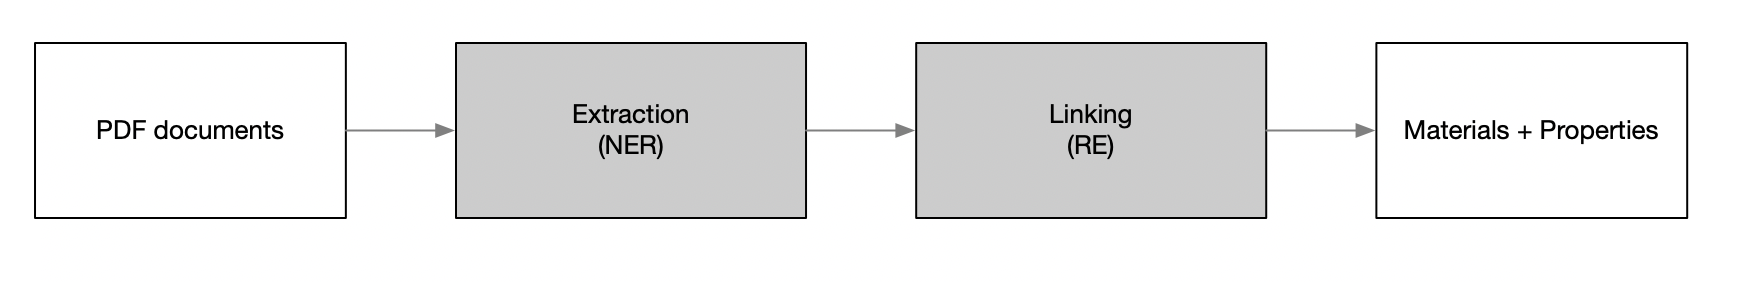
\includegraphics[width=\textwidth]{overview-schema}
\caption{Overview of the architecture}
\end{figure}

\subsubsection{Document structuring and pre-processing}
The Document structuring and pre-processing component processes the PDF document into a internal model structured as a list of text sentences.

% Internal process
The input document is processed using Grobid native models as illustrated in Figure~\ref{fig:grobid-document-processing}. After being transformed in XML by \textit{pdfalto}, it is passed to the "segmentation model" for recognising the macro areas (header, body and annex). As a result, the obtained sections are passed to specialised models in a cascade architecture. The header is further processed by the Header model, which further extracts the structure. We selectively extract title, abstract, keywords, publisher, publication year, doi and ignore other items, such as authors, publication date. 
Body and annexes are processed by the "Fulltext" model that recognises paragraphs, reference markers (decorations (also called \textit{reference callout}) in the text referring to the citation references at the end of the paper), tables and figure zones.
Tables and figures zones are further decomposed by the respective models and we retain only the caption text. 

\begin{figure}[ht]
\label{fig:grobid-document-processing}
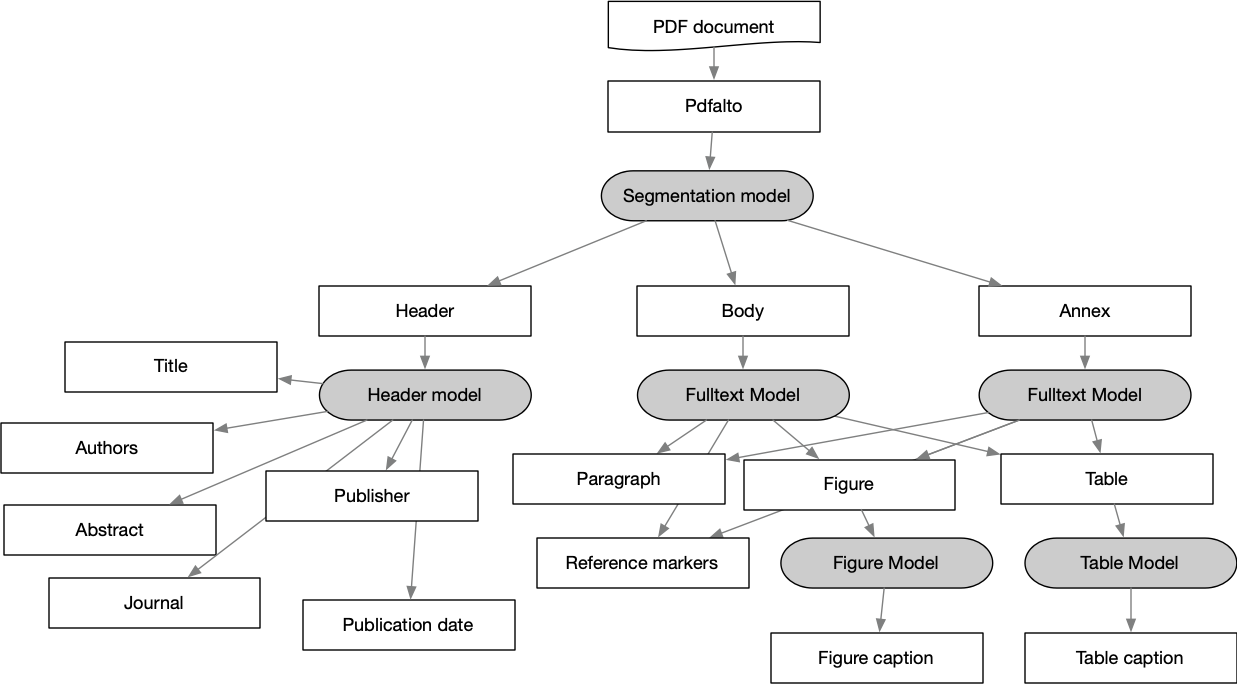
\includegraphics[width=\textwidth]{grobid-extraction-schema}
\caption{Cascade architecture in the document structuring with Grobid.}
\end{figure}

The text is finally passed to a sentence segmenter (we use Apache OpenNLP (\url{https://opennlp.apache.org})) which splits paragraphs into sentences. We use the reference markers collected from the text improve the sentence segmentation process: the segmentation is cancelled if the end of sentence falls within the boundaries of one reference marker. For example is often the case that a reference in the form of \textit{Foppiano et. al.} is mistakenly recognised as the end of the sentence. This method is very effective to enhance sentence segmentation in scientific text. 
The sentences are accumulated into special objects that represent general text passages containing the following properties: 
\begin{itemize}
    \item \textit{LayoutTokens} represent the token with layout information, such as style (italic, bold, superscript, and subscript), font (font type, font size), positions (coordinates (a list of pairs x,y), index position within the text chain), 
    \item \textit{section} contains the main sections: header, body and annex as they are divided from the Grobid "document segmentation model", 
    \item \textit{subsection} contains further division within the same section: paragraph, table or figure caption, abstract, title, 
    \item \textit{spans} are allocated to carry the extracted entities in the following step. One \textit{span} represents one entity with its type and position within the text. Spans can also store additional attributes using a key-value approach. For example a T\textsubscript{c} is represented by their form in the text but we can attach additional formats, for example their normalised representation. 
\end{itemize}

During the \textit{Document structuring and pre-processing}, the process extracts also the bibliographic data of the paper by combining the extracted information with a matching service to consolidate them against CrossRef\footnote{\url{https://www.crossref.org}}. In this way we ensure that the bibliographic data can match the publisher's information even if the paper was obtained from different sources, such as ArXiv. We collect the following bibliographic: title, authors, DOI, publisher, journal, and year of publication.

The following step of Extraction and Linking are enriching the internal structure by attaching additional structured information. 

\textbf{---- Revised till here -- following is WIP!}

\subsubsection{Extraction}

The second step in the architecture is the \textit{Extraction}, a named entities recognition (NER) from text. 
We designed this component as aggregation of multiple parsers focused on specific extractions and combining multiple machine learning models and rule-based algorithms.
The machine learning models can be trained using multiple architectures thanks to the integration with Grobid and the DeLFT (Deep Learning For Text) library~\cite{DeLFT}. 
We provides models for Conditional Random Field (CRF), Recurrent Neural Networks (RNN) using Bidirectional LSTM with CRF (BidLSTM\_CRF~\cite{Lample2016NeuralAF}), and Transformers (SciBERT~\cite{Beltagy2019SciBERT}).
The rule-based parsers are implemented using SpaCy (\url{https://spacy.io} entity ruler.

Figure~\ref{fig:extraction-ml-models-cascade-architecture} illustrates the data flow, the interaction of the parsers and the output information. We describe in details in the following paragraphs.  

\begin{figure}[ht]
\label{fig:extraction-ml-models-cascade-architecture}
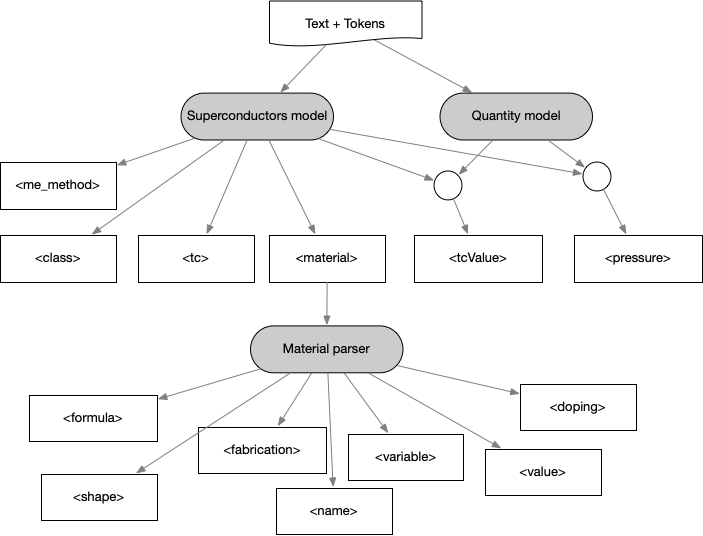
\includegraphics[width=\textwidth]{extraction-schema-2}
\caption{Cascade architecture combining the superconductors and material parsers.}
\end{figure}

\paragraph{Superconductors parser} combines two ML models (superconductors and quantities) and three RB extractors. The former was trained using SuperMat and aims to extract the main entities \texttt{<material>}, \texttt{<tcValue>}, T\textsubscript{c} expressions \texttt{<tc>}, \texttt{<pressure>}, measurement methods \texttt{<me\_method>} while the latter focuses only on quantities, in particular temperature and pressures. The pressures and temperatures that are overlapping between the two models are merged by prioritizing the largest matches. Trained with data from SuperMat~\cite{foppiano2021supermat} with evaluation results in Table~\ref{tab:evaluation-10fold-superconductors-parser}.

\paragraph{material parser} is used to further decompose \texttt{<material>} entities into additional attributes such as doping, formula and so on. The material parser also uses additional techniques to decompose formula into composition and to transform name into formula (e.g. hydrogen in H). In addition when a material is in the stochiometric form and it contains the substitution variables, the material parser tries to substitute and create n formula using permutation. For example the stochiometric formula \texttt{La 4 Fe 2 A 1-x O 7 (A=Mg,Co; x=0.1,0.2)} will permute the values of A and x to obtain \texttt{La 4 Fe 2 Mg 0.9 O 7}, \texttt{La 4 Fe 2 Mg 0.8 O 7}, \texttt{La 4 Fe 2 Co 0.9 O 7}, \texttt{La 4 Fe 2 Co 0.8 O 7}. Trained with data from SuperMat~\cite{foppiano2021supermat} and its results are available in Table~\ref{tab:evaluation-10fold-material-parser}. Since the performances with CRF or RNN are above 90\%, we do not supply the model based on transformers for this task. 

\paragraph{quantities parser} from the project \textit{grobid-quantities}~\cite{foppiano2019quantities} and trained on scientific text. This model is trained to extract any type of quantities of measurement. We keep only temperatures and pressures and we merge the entities that are partially or completely overlapping with the superconductors \texttt{<tcValue>} or \texttt{<pressure>} entities and we keep the largest matches. 

It recognises nine type of entities synthesised in Table~\ref{tab:superconductors-model-entities}, the entities extracted by machine learning are described more in details in~\cite{foppiano2021supermat}.

\begin{table}[ht]
\centering
\begin{tabular}{m{10em} m{25em}}
\hline 
\textbf{Entity} (\textbf{Tag})& \textbf{Description} \\ 
\hline
\hline
\multicolumn{2}{c}{\textbf{Machine learning}} \\
\hline
Material (\texttt{<material>}) & Materials and samples names, formulas, including stochiometric formulas, substitution variables of values and elements, shape, doping, substrate \\
Class (\texttt{<class>}) & Groups of materials having similar characteristics or common strategic compounds that define their nature \\
T\textit{c} value (\texttt{<tcValue>})& \\
T\textit{c} expressions (\texttt{<tc>}) & Expressions in the text that provide information about the phenomenon of superconductivity related to a value, interval or variation of the T\textsubscript{c}\\
Measurement methods (\texttt{<me\_method>}) & Techniques used to measure or calculate the presence of superconductivity. \\
Applied pressure (\texttt{<pressure>}) & Applied pressure when superconductivity is recorded\\
\hline
\hline
\multicolumn{2}{c}{\textbf{Rule-based}} \\
\hline
Crystal structure & Geometry of arrangement of particles in the unit cell\\
Space groups  & Symmetry group, usually in three dimensions\\
Unit cells & A repeating unit formed by the vectors spanning the points of a lattice\\
\hline
\end{tabular}
\label{tab:superconductors-model-entities}
\caption{Synthesis of the superconductors parser entities. }
\end{table}

The \textit{Extraction} is also designed with a cascade architecture: entities of type \texttt{<materials>} are further decomposed into \texttt{<formula>}, \texttt{<name>}, \texttt{<substrate>}, \texttt{<fabrication>}, \texttt{<value>} and \texttt{<variables>}, \texttt{<doping>}, \texttt{<shape>} as illustrated in Figure~\ref{fig:extraction-ml-models-cascade-architecture}.

They implements the following models: 


 for extracting finite set of crystal structure, space groups and unit cells. The space groups are taken from the list in Wikipedia\footnote{\url{https://en.wikipedia.org/wiki/List_of_space_groups}}. This component will be integrated in the SuperMat corpus in future to improve the tolerance to noise. 

\begin{table}[ht]
\centering
\scalebox{0.7}{
\begin{tabular}{l|ccc|ccc|ccc}
& \multicolumn{3}{c}{\textbf{CRF}} & \multicolumn{3}{c}{\textbf{BidLSTM+CRF} (RNN)} & \multicolumn{3}{c}{\textbf{SciBERT} (transformers)}\\ 
\textbf{Label} & \textbf{Precision} & \textbf{Recall} & \textbf{F1} & \textbf{Precision} & \textbf{Recall} & \textbf{F1} & \textbf{Precision} & \textbf{Recall} & \textbf{F1} \\ \hline
\texttt{<class>}         & 79.69 & 75.54 & 77.55 & 81.84 & 83.96 & 82.85 & 79.58 & 85.79 & 82.56\\
\texttt{<material>}      & 82.9  & 81.33 & 82.1  & 85.18 & 83.86 & 84.51 & 83.89 & 86.13 & 84.99\\
\texttt{<me\_method>}    & 82.47 & 81.26 & 81.84 & 83.51 & 83.37 & 83.43 & 83.92 & 86.50 & 85.19\\
\texttt{<pressure>}      & 65.03 & 54.01 & 58.26 & 63.79 & 73.24 & 67.98 & 63.92 & 71.18 & 67.27\\
\texttt{<tc>}            & 84.63 & 80.73 & 82.63 & 83.70 & 81.66 & 82.66 & 80.91 & 83.00 & 81.94\\
\texttt{<tcValue>}       & 79.3  & 74.95 & 76.97 & 73.23 & 80.73 & 76.76 & 76.74 & 85.00 & 80.65\\
\hline
All (micro avg) & 82.43 & 79.68 & 81.03 & \textbf{83.01} & 82.89 & 82.95 & 83.01 & \textbf{85.06} & \textbf{83.46}\\
\hline
\end{tabular}
}
\caption{Evaluation scores for the superconductor models using 10-fold cross-validation. }
\label{tab:evaluation-10fold-superconductors-parser}
\end{table}


\begin{table}[ht]
\centering
\begin{tabular}{l|ccc|ccc}
& \multicolumn{3}{c}{\textbf{CRF}} & \multicolumn{3}{c}{\textbf{BidLSTM+CRF} (RNN)}\\ 
\hline \textbf{Label} & \textbf{Precision} & \textbf{Recall} & \textbf{F1} & \textbf{Precision} & \textbf{Recall} & \textbf{F1} \\ \hline

\texttt{<doping>}      & 86.31   & 86.2     & 86.22 & 84.87 &  87.82 & 86.29   \\
\texttt{<fabrication>} & 60.93   & 50.3     & 54.27 & 7.43  &  13.33 & 8.94   \\
\texttt{<formula>}     & 98.06   & 97.93    & 98    & 97.33 &  97.51 & 97.42  \\
\texttt{<name>}        & 97.25   & 96.95    & 97.09 & 96.08 &  96.70 & 96.38  \\
\texttt{<shape>}       & 97.26   & 97.15    & 97.2  & 96.38 &  94.93 & 95.64  \\
\texttt{<substrate>}   & 83.33   & 60.83    & 68    & 65.76 &  97.50 & 77.66  \\
\texttt{<value>}       & 95.99   & 95.99    & 95.99 & 95.28 &  95.84 & 95.56  \\
\texttt{<variable>}    & 99.24   & 98.85    & 99.04 & 98.94 &  98.99 & 98.96  \\
\hline
all  (micro avg)       & 96.87   & 96.51    & 96.68  & 95.75 &   96.44  &  96.09  \\
\hline
\end{tabular}
\caption{Evaluation scores of 10-fold cross-validation of the material parser. }
\label{tab:evaluation-10fold-material-parser}
\end{table}

In Table~\ref{tab:evaluation-10fold-superconductors-parser} and~\ref{tab:evaluation-10fold-material-parser} we illustrate the evaluation scores for the superconductors and materials parsers models using 10-fold cross-validation. 
The superconductors parser (Table~\ref{tab:evaluation-10fold-superconductors-parser}) best result was achieved using transformers, in particular SciBERT had a F1 score of 83.46\% and recall around 85\%. It's worth noticing that the SciBERT approach is the slowest to comupute and requires a server with a proper GPU.
However, the BidLSTM+CRF (RNN) had the best trade-off between performances and throughput, as compared with the SciBERT approach. 

We notice that \texttt{<pressure>} results in lower performances and the reason due to the lack of enough training data as compared with the rest of the labels. 

The materials parser is provided in two architectures: CRF and BidLSTM+CRF because the performances are above 95\% and SciBERT approach is very slow. 
In this model \texttt{<fabrication>} and \texttt{<substrate>} have relatively low results, for the same reason of \texttt{<pressure>} of lack of enough training data.
[PO we can potentially extend this part adding an additional section discussing NER]

\subsubsection{Linking}

%Introduction of the linking
The Linking is the step that aims to link together entities previously extracted.
%Objective of the linking
We can formalised it as follows. \textit{Given a text T and two or more entities e\textsubscript{1}...e\textsubscript{n} of two types t\textsubscript{1} and t\textsubscript{2}, determine links between entities of type t\textsubscript{1} can be linked to entities of type t\textsubscript{2} .} 

We have experimented several options: dependency parsing, rule-based, and sequence labelling. 
Our implementation uses a main rule-based method and a secondary approach based on sequence labelling. The dependency parsing was studied using several approaches from scientific literature~\cite{yoshikawa:2017acl, Tiktinsky2020pyBARTES, swayamdipta:17, zhou-zhao-2019-head} and it was discarded. We found two main reasons a) the difficulty to find parser that were trained or performing on scientific text, and, by consequence, b) the implementation was converging toward a complex set of rules which were compensating for the poor performances on the dependency parser.

% Algorithm in brief (three or four different scenario): 
\paragraph{T\textsubscript{c} classification}
For linking the T\textsubscript{c} to any other entity type, there is an additional step to classify the temperature into "superconducting" or "non-superconducting" critical temperatures. 
The classification is rule-based and combines the extracted entities of T\textsubscript{c} expressions (label \texttt{<tc>}) with a set of predefined standard names. 
If a T\textsubscript{c} is not considered a "superconducting critical temperature", it's excluded from the list of possible linking candidates. 

\paragraph{Rule-based linking}
The rule-based approach works with two main scenarios: a) when entities to be linked have cardinality one they are linked automatically, and b) when they have higher cardinality they are linked "by distance" or "in order", depending on the structure of the sentence. 
If the word \textit{"respectively"} appears in the sentence, entities are linked "in order", otherwise they are linked "by distance". 
For example, the sentence containing the word "respectively":  
\begin{displayquote}
P-or Ba-122  and Co-doped Ba-122 have lower T c s of about 30 K and 24 K, respectively, which makes helium free operation questionable.
\end{displayquote}
is processed linking the materials in order: \textit{P-or Ba122} is assigned to \textit{30 K} and \textit{Co-doped Ba-122} to \textit{24 K}.
The "in order" method is very sensible to missing entities, for example if one entity is not extracted by mistake it will incorrectly assign all the entities in the block. To avoid this, if the entities are unbalanced we reduce the search space as follows: 
\begin{itemize}
    \item 3 entities of type\textsubscript{1} vs 2 entities of type\textsubscript{2}: we shift the starting point to start at the second entity 
    \item 2 entities of type\textsubscript{1} vs 3 entities of type\textsubscript{2}: we shift the ending point at the n\textsubscript{-1} entity
\end{itemize}
In this way we avoid that the entities in surplus are just ignored. 

We define the distance measurement \textit{d} calculated in characters, from the centre of the entities. The entity can be expanded if surrounded by parenthesis, and centre can be adjusted. Since the parenthesis become a block on itself, all its content refers to the same entity. 
As an example, in the sentence
\begin{displayquote}
We tested two materials MgB2 (Tc = 39K) and LaFe (Tc = 16K).
\end{displayquote}
both temperatures are expanded to their containing parenthesis \texttt{39K} to \texttt{(Tc = 39K)}, moving the centre toward the left. As a result, the distance tend to be shorter to entities immediately closed to the whole parenthesis block. Moreover, the impact of the dimension of the whole parenthesis block is reduced when calculating the distance. 

The distance calculation is also adjusted with the addition of "penalties", that is, the distance is doubled when certain keywords such as "and", ", ", "." representing logical separation of predicates appear in the sentence. The rationale is that element between two separated predicates are likely not to be linked although they might be at a smaller distance. 

\paragraph{Sequence labelling linking} We designed the linking based on sequence labelling as a simple task where each token has been assigned two possible labels: \texttt{<link\_left>} or \texttt{<link\_right>}. The post-processing decodes the labels and translated them into linking between entities. 
This approach has a obvious limitation to linking subsequent entities.  

\paragraph{Results} In our implementation we focus on three types of relationships: 
\begin{itemize}
    \item \textbf{material-tcValue} links a material with its corresponding superconducting critical temperature value, 
    \item \textbf{tcValue-pressure} connects a superconducting critical temperature value with its related critical pressure, and 
    \item \textbf{me\_method-tcValue} connects the superconducting critical temperature value to its corresponding measurement method.
    % \item \textbf{material-crystal\_structure} link the material with their crystal structure, and 
    % \item \textbf{material-space\_group} to link the material to their space groups.
\end{itemize}

The evaluation is shown in Table \ref{table:evaluation-linking}. 
The rule-based was tested using the SuperMat~\cite{foppiano2021supermat} corpus which contains linked entities. Each test was framed to test the linking between two entities type. 
The result of the \texttt{material-tcValue} obtained above 80\% F1 score with a precision of 88\%. We would like to stress we strive to obtain higher precision scores. 

The approach with sequence labelling was less performant, with scores of 69.16\%, 69.76\%, and 44.65\% F1 score, respectively. In general, the effectiveness of this methodology is dubious, however the amount of training data that can be used is smaller than for NER. 
This is the main cause of the lower score of \texttt{tcValue-me\_method}. 


\begin{table}[ht]
\centering
\begin{tabular}{lccc}
\hline \textbf{Linked entities} (Method) & \textbf{Precision} & \textbf{Recall} & \textbf{F1-score} \\ \hline
\textbf{material-tcValue} (Rule-based)  & 88.00 	&   74.00      &	81.00      \\
\textbf{material-tcValue} (CRF)         & 68.52 &	70.11   &  69.16    \\
\textbf{tcValue-pressure} (CRF)         & 72.92 &	67.67   &  69.76    \\
\textbf{tcValue-me\_method} (CRF)       & 49.99 &	45.21   &  44.65   \\
\hline
\end{tabular}
\label{table:evaluation-linking}
\caption{Evaluation scores of the linking methods. }
\end{table}

\subsection{End to end evaluation}

What is the end 2 end evaluation? 
How the end 2 end evaluation is performed? 

Discussion of the results, which problems are currently emerging what are the prospective for the future?

\begin{table}[ht]
\centering
\begin{tabular}{lccc}
\hline \textbf{Precision} & \textbf{Recall} & \textbf{F1-score} & \textbf{Support} \\ \hline
73.86  &	66.33 &	69.90 & 597\\
\hline
\end{tabular}
\label{table:end2end-evaluation}
\caption{End 2 end evaluation scores. }
\end{table}

\section{Supercon\textsuperscript{2}}

Introduction of the database, which data was extracted and the format 

\subsection{Ingestion workflow}
\label{subsec:ingestion-workflow}

\begin{figure}[ht]
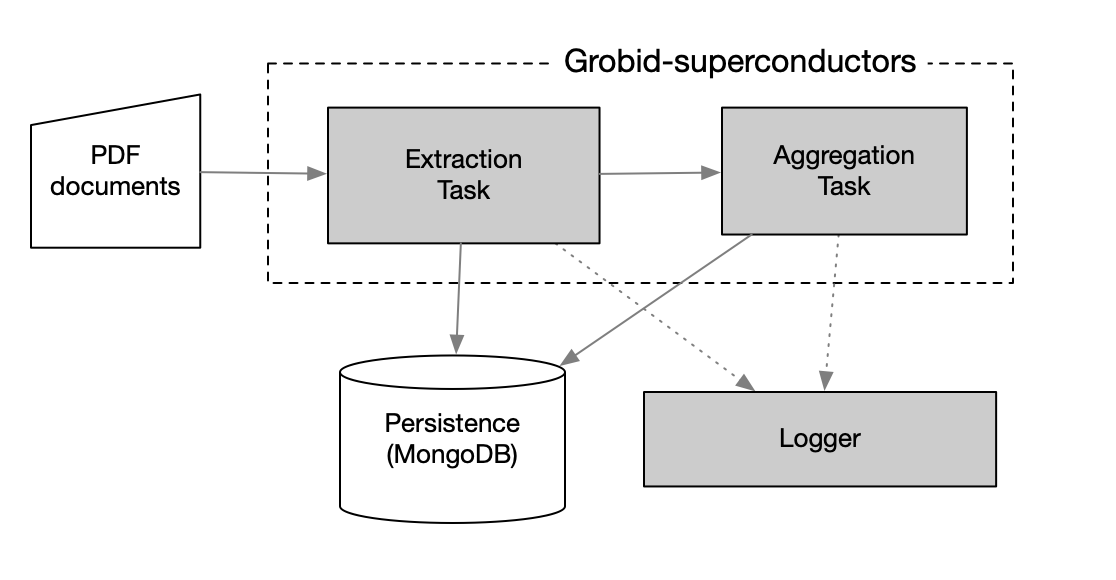
\includegraphics[width=\textwidth]{workflow-schema-1}
\caption{Schema of the ingestion workflow}
\end{figure}


Quickly discussion on the ingestion workflow 


\subsection{User interface}
\label{sucsec:supercon2-user-interface}


\section{Conclusion}
\label{sec:conclusion}

\bibliography{bibliography}
\bibliographystyle{plain}


\end{document}
